\documentclass[10pt]{report}
\usepackage[utf8]{inputenc}
\usepackage{amsfonts}
\usepackage{amsmath}
\usepackage{amssymb}
\usepackage{commath}
\usepackage[ngerman]{babel}
\usepackage{enumitem}
\usepackage{booktabs}
\usepackage{longtable}
\usepackage{relsize}
\usepackage{pgfplots}
\usepackage{csvsimple}
\usepackage{pgfplotstable}
\usepackage{siunitx}
\usepackage{fancyhdr}
\usepackage{color}
\usepackage{float}

\setlength\parindent{0pt}

\setcounter{chapter}{3}

\pagestyle{fancy}
\fancyhf{}
\lhead{GPET Versuch 2}
\rhead{Tim Luchterhand, Paul Nykiel}
\cfoot{\thepage}

\author{Tim Luchterhand, Paul Nykiel}
\title{GPET Versuch 2}

\begin{document}
        \maketitle

        \section{Bestimmung des Innenwiderstandes einer Quelle}
        \textbf{Aufgabe:} Nehmen Sie die Strom-Spannungskennlinie der Batterie auf. Verwenden sie hierzu Messtabelle
        1 und tragen Sie die Messwerte in ein Diagramm ein. Schließen Sie das Spannungsmessgerät
        vor der Batterie an, damit Sie die Batterie nicht über einen längeren
        Zeitraum kurzschließen.

        \begin{equation*}
            U_{innen} = U_{Batterie} - U_{mess}
        \end{equation*}

        % TODO Messwerte quelleWiderstand.csv
        \begin{table}[h!]
            \begin{center}
                \caption{Messtabelle für Versuch 1}
                \label{tablec}
                \pgfplotstabletypeset[
                multicolumn names, % allows to have multicolumn names
                col sep=space, % the seperator in our .csv file
                display columns/0/.style={
                column name=$R_L$, % name of first column
                column type={S},string type},  % use siunitx for formatting
                display columns/1/.style={
                column name=$U_{mess}$,
                column type={S},string type},
                display columns/2/.style={
                column name=$U_{innen}$,
                column type={S},string type},
                display columns/3/.style={
                column name=$I_L$,
                column type={S},string type},
                every head row/.style={
                before row={\toprule}, % have a rule at top
                after row={
                \si{\ohm} & \si{\volt} & \si{\volt} & m\si{\ampere}\\
                \midrule} % rule under units
                },
                every last row/.style={after row=\bottomrule},
                ]{quelleWiderstand.csv}
            \end{center}
        \end{table}

        \subsection{U-I-Diagram}
        \begin{center}
            \begin{tikzpicture}
        		\begin{axis}[ymin=0, xmin=0, xlabel = {$U_{innen}$[V]}, ylabel = {$I_L$[mA]}]
        			\addplot[color=blue] table[x index = {2},
                            y index = {3}] {quelleWiderstand.csv};
        		\end{axis}
        	\end{tikzpicture}
        \end{center}

        \subsection{Charakterisierung der Ersatzspannungsquelle}
        \textbf{Aufgabe:} Charakterisieren Sie die Ersatzspannungsquelle mit Hilfe des erstellten Diagramms.

        \vspace{0.5cm}

        %TODO Erklärung
        Die Steigung des Graphens ist der Innenwiderstand $R_{innen}$. Es gilt
        \begin{equation*}
            R_{innen} = \frac{(U_{Batterie} - U_{mess})(R+R_L)}{U_{mess}}
        \end{equation*}

        \section{Untersuchung eines einfachen Netzwerks}
        Bauen Sie die Schaltung aus Abbildung 6 nach. Die Widerstandswerte sind $R1 = R2 =
        1 \si{\ohm}$ und $R3 = R4 = 100\si{\ohm}$.

        Bestimmen Sie die äquivalente Ersatzspannungsquelle zwischen den Knoten 0 und 1 durch
        Messung ($U_{in} = 3\si{\volt}$). Verwenden Sie hierzu wieder das Potentiometer mit $1\si{k\ohm}$ und tragen
        Sie die Ergebnisse in Messtabelle 2 ein.

        %TODO Messwerte einfachesNetzwerk.csv
        \begin{table}[h!]
            \begin{center}
                \caption{Messtabelle für Versuch 2}
                \label{tableb}
                \pgfplotstabletypeset[
                multicolumn names, % allows to have multicolumn names
                col sep=space, % the seperator in our .csv file
                display columns/0/.style={
                column name=$R_L$, % name of first column
                column type={S},string type},  % use siunitx for formatting
                display columns/1/.style={
                column name=$U_{mess}$,
                column type={S},string type},
                display columns/2/.style={
                column name=$I_L$,
                column type={S},string type},
                every head row/.style={
                before row={\toprule}, % have a rule at top
                after row={
                \si{\ohm} & m\si{\volt} & m\si{\ampere}\\
                \midrule} % rule under units
                },
                every last row/.style={after row=\bottomrule},
                ]{einfachesNetzwerk.csv}
            \end{center}
        \end{table}

        \subsection{Ersatzspannungsquelle}
        \subsubsection{Arbeitsgerade}
        \begin{center}
            \begin{tikzpicture}
        		\begin{axis}[ymin=0, xmin=0, xlabel = {V}, ylabel = {mA}]
        			\addplot[color=blue] table[x index = {1},
                            y index = {2}] {einfachesNetzwerk.csv};
        		\end{axis}
        	\end{tikzpicture}
        \end{center}

        %TODO Ersatzspannungsquelle bestimmen
        Berechnung des Kurzschlussstroms durch lineare Regression:
        \begin{eqnarray*}
            U_{Quelle} &=& \si{\volt}\\
            I_{Kurzschluss} &=& \si{\ampere}\\
            R_{Innen} &=& \si{\ohm}
        \end{eqnarray*}


        \subsection{Widerstand}
        \textbf{Aufgabe:} Messen Sie die Spannungen an den Widerständen in Abhängigkeit von $U_{in}$. Tragen Sie
        die Messwerten in Messtabelle 3 ein und vergleichen diese mit den berechneten Werten in
        einem Diagramm.
        %TODO Messwerte quelleWiderstand2.csv
        \begin{table}[h!]
            \begin{center}
                \caption{Messtabelle für Versuch 2}
                \label{tablec}
                \pgfplotstabletypeset[
                multicolumn names, % allows to have multicolumn names
                col sep=space, % the seperator in our .csv file
                display columns/0/.style={
                column name=$U_{in}$, % name of first column
                column type={S},string type},  % use siunitx for formatting
                display columns/1/.style={
                column name=$U_{R1,soll}$,
                column type={S},string type},
                display columns/2/.style={
                column name=$U_{R2,soll}$,
                column type={S},string type},
                display columns/3/.style={
                column name=$U_{R3,soll}$,
                column type={S},string type},
                display columns/4/.style={
                column name=$U_{R4,soll}$,
                column type={S},string type},
                display columns/5/.style={
                column name=$U_{R1,mess}$,
                column type={S},string type},
                display columns/6/.style={
                column name=$U_{R2,mess}$,
                column type={S},string type},
                display columns/7/.style={
                column name=$U_{R3,mess}$,
                column type={S},string type},
                display columns/8/.style={
                column name=$U_{R4,mess}$,
                column type={S},string type},
                every head row/.style={
                before row={\toprule}, % have a rule at top
                after row={
                \si{\volt} & \si{\volt} & \si{\volt} & \si{\volt} & \si{\volt} & \si{\volt} & \si{\volt} & \si{\volt} & \si{\volt}\\
                \midrule} % rule under units
                },
                every last row/.style={after row=\bottomrule},
                ]{quelleWiderstand2.csv}
            \end{center}
        \end{table}

        \subsection{Diagramm}
        Berechnete Werte in \textcolor{red}{rot}, gemessene Werte in \textcolor{blue}{blau}.
        \subsubsection{Vergleich $R_1$}
        \begin{center}
            \begin{tikzpicture}
        		\begin{axis}[ymin=0, xmin=0, xlabel = {$U_{in}$[V]}, ylabel = {$U_{R_1}$[V]}]
        			\addplot[color=red] table[x index = {0},
                            y index = {1}] {quelleWiderstand2.csv};
                    \addplot[color=blue] table[x index = {0},
                            y index = {5}] {quelleWiderstand2.csv};
        		\end{axis}
        	\end{tikzpicture}
        \end{center}
        \subsubsection{Vergleich $R_2$}
        \begin{center}
            \begin{tikzpicture}
                \begin{axis}[ymin=0, xmin=0, xlabel = {$U_{in}$[V]}, ylabel = {$U_{R_2}$[V]}]
        			\addplot[color=red] table[x index = {0},
                            y index = {2}] {quelleWiderstand2.csv};
                    \addplot[color=blue] table[x index = {0},
                            y index = {6}] {quelleWiderstand2.csv};
        		\end{axis}
        	\end{tikzpicture}
        \end{center}
        \subsubsection{Vergleich $R_3$}
        \begin{center}
            \begin{tikzpicture}
                \begin{axis}[ymin=0, xmin=0, xlabel = {$U_{in}$[V]}, ylabel = {$U_{R_3}$[V]}]
        			\addplot[color=red] table[x index = {0},
                            y index = {3}] {quelleWiderstand2.csv};
                    \addplot[color=blue] table[x index = {0},
                            y index = {7}] {quelleWiderstand2.csv};
        		\end{axis}
        	\end{tikzpicture}
        \end{center}
        \subsubsection{Vergleich $R_4$}
        \begin{center}
            \begin{tikzpicture}
                \begin{axis}[ymin=0, xmin=0, xlabel = {$U_{in}$[V]}, ylabel = {$U_{R_4}$[V]}]
        			\addplot[color=red] table[x index = {0},
                            y index = {4}] {quelleWiderstand2.csv};
                    \addplot[color=blue] table[x index = {0},
                            y index = {8}] {quelleWiderstand2.csv};
        		\end{axis}
        	\end{tikzpicture}
        \end{center}

        \section{Untersuchung eines komplizierten Netzwerks}
        \textbf{Aufgabe:} Messen Sie die Spannungen an allen
        Knoten in Abhängigkeit von $U_{in,1} = 0 \ldots 3 \si{\volt}$ und tragen Sie die Ergebnisse in Messtabelle
        4 ein. Erstellen Sie ein Diagramm für die Spannungen an allen Knoten in Abhängigkeit
        der Spannung $U_{in,1} = 0 \ldots 3 \si{\volt}$.
        %TODO Messwerte kompliziertesNetzwerk.csv
        \begin{table}[h!]
            \begin{center}
                \caption{Messtabelle für Versuch 3}
                \label{tablec}
                \pgfplotstabletypeset[
                multicolumn names, % allows to have multicolumn names
                col sep=space, % the seperator in our .csv file
                display columns/0/.style={
                column name=$U_{in,1}$, % name of first column
                column type={S},string type},  % use siunitx for formatting
                display columns/1/.style={
                column name=$U_{1,mess}$,
                column type={S},string type},
                display columns/2/.style={
                column name=$U_{2,mess}$,
                column type={S},string type},
                display columns/3/.style={
                column name=$U_{3,mess}$,
                column type={S},string type},
                display columns/4/.style={
                column name=$U_{4,mess}$,
                column type={S},string type},
                every head row/.style={
                before row={\toprule}, % have a rule at top
                after row={
                \si{\volt} & \si{\volt} & \si{\volt} & \si{\volt} & \si{\volt}\\
                \midrule} % rule under units
                },
                every last row/.style={after row=\bottomrule},
                ]{kompliziertesNetzwerk.csv}
            \end{center}
        \end{table}

        \subsection{Diagramm der Knotenspannungen}
        \begin{center}
            \begin{tikzpicture}
        		\begin{axis}[ymin=0, xmin=0, xlabel = {V}, ylabel = {mA}]
        			\addplot[color=red] table[x index = {0},
                            y index = {1}] {kompliziertesNetzwerk.csv};
                    \addplot[color=blue] table[x index = {0},
                            y index = {2}] {kompliziertesNetzwerk.csv};
                    \addplot[color=green] table[x index = {0},
                            y index = {3}] {kompliziertesNetzwerk.csv};
                    \addplot[color=black] table[x index = {0},
                            y index = {4}] {kompliziertesNetzwerk.csv};
        		\end{axis}
        	\end{tikzpicture}
        \end{center}

        \subsection{Knotenpotenzialanalyse mit Matlab}
        \textbf{Aufgabe:} Nun soll für dieses Netzwerk das in Abschnitt 2.2 aufgestellte KPV mit Hilfe von Matlab
        gelöst und mit den Ergebnissen der eben durchgeführten Messungen verglichen werden.

        \vspace{0.5cm}

        %TODO Matlab, Screenshot?
        %\begin{figure}[H]
        %  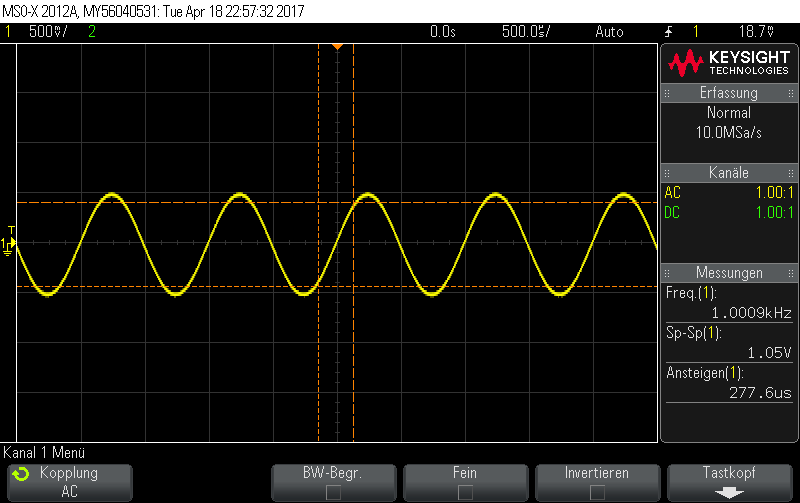
\includegraphics[width=\textwidth]{scope_5.png}
        %  \caption{DC}
        %\end{figure}

        \section{Aufbau einer Messbrücke nach Wheatstone}
        \textbf{Aufgabe:} Kann mit diesem Messaufbau jeder Widerstand gemessen werden? Falls dies nicht der
        Fall ist, wie muss der Messaufbau verändert werden, damit die restlichen Widerstände
        gemessen werden können?

        \vspace{0.5cm}

        %TODO Text

\end{document}
